%%%%%%%%%%%%%%%%%%%%%%%%%%%%%%%%%%%%%%%%%%%%%%%%%%%%%
%%% Courseware for a Short Course in R programming
%%%%%%%%%%%%%%%%%%%%%%%%%%%%%%%%%%%%%%%%%%%%%%%%%%%%%
%

\mode<article>{\maketitle \tableofcontents\vfil \newpage }
\mode<presentation>{\begin{frame}
\vss
$$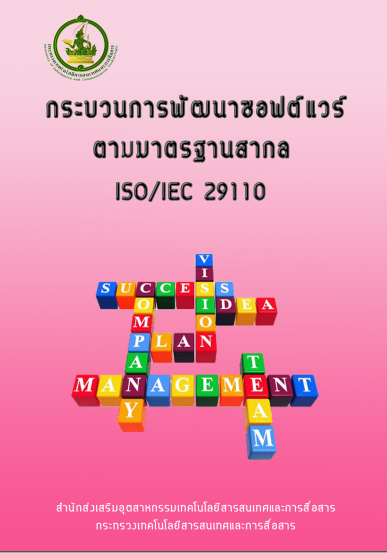
\includegraphics[width=.2\textwidth]{mictmanual.png}$$
\vss
    \titlepage
    \end{frame}
    \begin{frame}[allowframebreaks]
        \frametitle{Outline of this session}
        \tableofcontents
    \end{frame}}    
    
\section{Background to ISO 29110}
\begin{frame}{Human nature}
\begin{itemize}
\item Distractable
\item Forgetful
\item Mind fills in the holes
\end{itemize}
\bigskip
\url{https://www.youtube.com/watch?v=xcUOTrlpSuI}
\end{frame}

\begin{frame}{Consequence of Human Fragility}
$$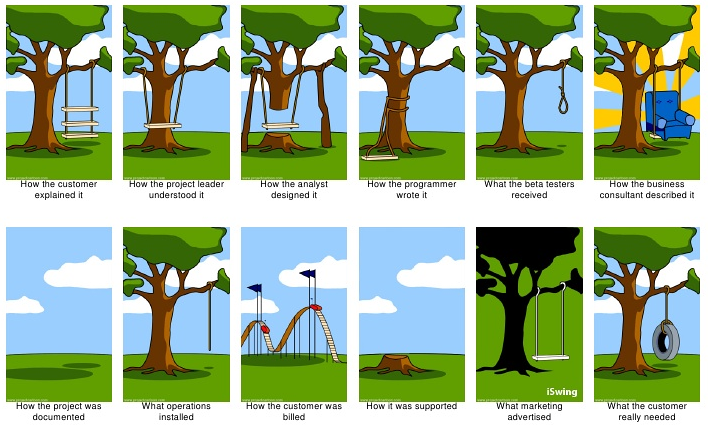
\includegraphics[width=.9\textwidth]{swing.png}$$
\end{frame}

\begin{frame}{ISO Standards}
\kern -.3in
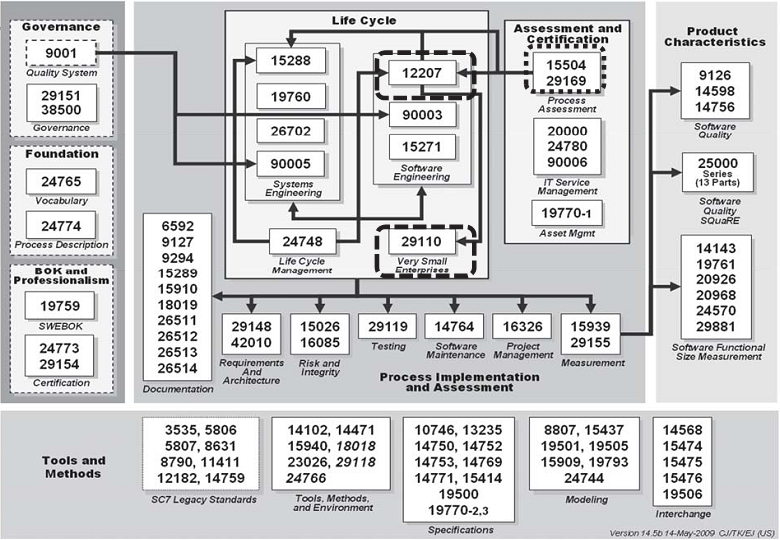
\includegraphics[width=.9\textwidth]{isohistory.png}
\end{frame}

\begin{frame}{ISO Standards for Lifecycle Management}
\kern -.2in
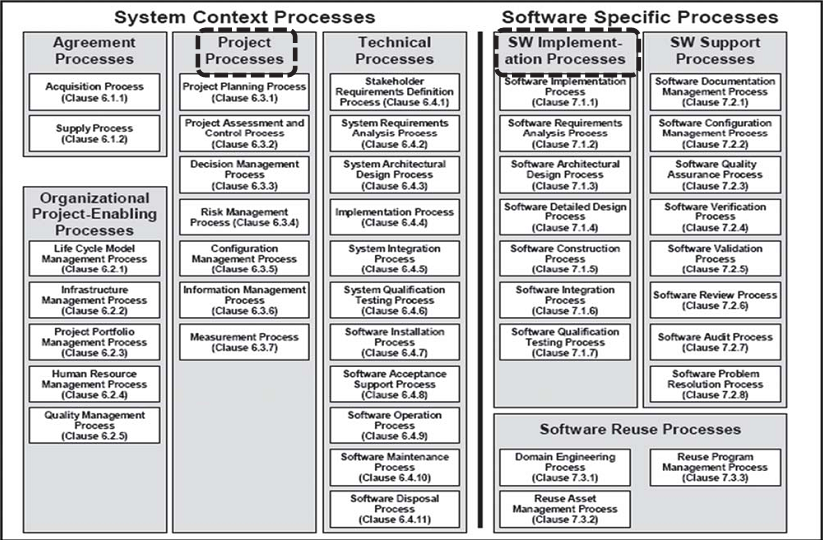
\includegraphics[width=.85\textwidth]{isolifecycle.png}
\end{frame}

\section{Growing Support for ISO29110}
\begin{frame}{Growing support for ISO 29110}
\kern -.3in
$$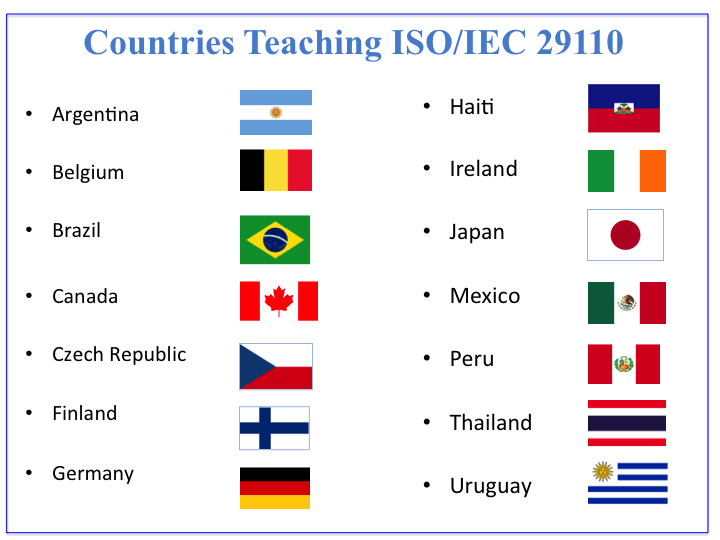
\includegraphics[width=.85\textwidth]{countries.png}$$
\end{frame}

\begin{frame}{Support for ISO29110}
\begin{columns}
\column{.3\textwidth}

\includegraphics[height=1.75in]{ministrylogo.png}
\column{.1in}
\relax
\column{.3\textwidth}

\includegraphics[height=1.75in]{iso.png}
\column{.1in}
\relax
\end{columns}
\end{frame}

\begin{frame}{Thai eBook on ISO 29110}
$$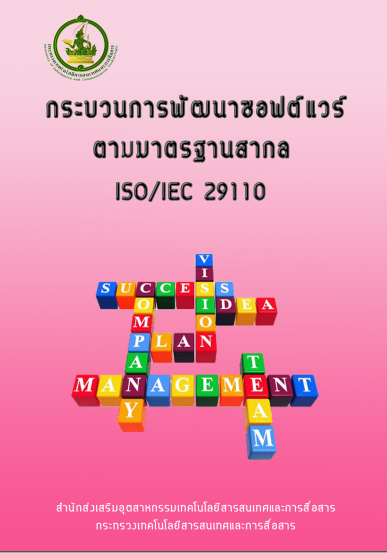
\includegraphics[width=.4\textwidth]{mictmanual.png}$$

\tiny
\url{http://www.mict.go.th/assets/portals/1/files/download/580820_eBook_ISO29110_MICT.pdf}
\end{frame}

\section{Comparision with CMMI}
\begin{frame}{CMMI vs ISO29110 Project Management}
$$\small
\begin{tabular}{p{2in}p{2in}}
CMMI & ISO 29110 \\
\hline
Project planning & Project planning \\
\hline
Project monitoring and control & Project plan execution \\
& Project assessment and control project closure \\
\hline
Requirement management & Change requests
\hline
Configuration management & Version Control Strategy \\
 & Configuration \\
\hline
Process and product quality assurance &
 Software quality assurance\\
 & Implement validation and review task performed\\
\hline
\end{tabular}
$$
\end{frame}

\begin{frame}{CMMI Engineering vs ISO29110 Software Implementation}
$$\small
\begin{tabular}{p{2in}p{2in}}
CMMI & ISO 29110 \\
\hline
Project planning & Software implementation \\
\hline
Requirements management & Software requirements analysis \\
Requirement development & \\
\hline
Technical solutions & Software architectural and detailed design \\
& Software construction \\
Requirements management & Prodcut delivery \\
 & Traceability to requirements \\
\hline
Verification & Software integration and tests \\
Validation & \\
\hline
\end{tabular}
$$
\end{frame}


\section{Project Management Processes}

\begin{frame}{Project Management}
\null
\kern -.5in
$$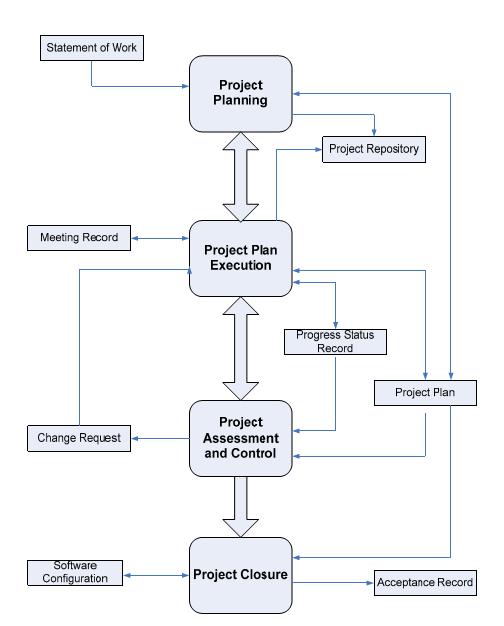
\includegraphics[width=.7\textheight]{PMprocess.png}$$
\end{frame}


\begin{frame}{Project Management}
\begin{itemize}
\item PM Input Products
\begin{itemize}
\item Statement of Work
\item Software Configuration
\item Change Requests
\end{itemize}
\item PM Internal Products
\begin{itemize}
\item Change Requests
\item Meeting Records
\item Progress Status Record
\end{itemize}
\item PM Output Products
\begin{itemize}
\item Project Plan
\item Acceptance Record
\item Project Repository
\item Meeting Record
\item Software Configuration
\end{itemize}
\end{itemize}
\end{frame}

\section{Software Implementation Processes}
\begin{frame}{Software Implementation}
\null
\kern -.75in
$$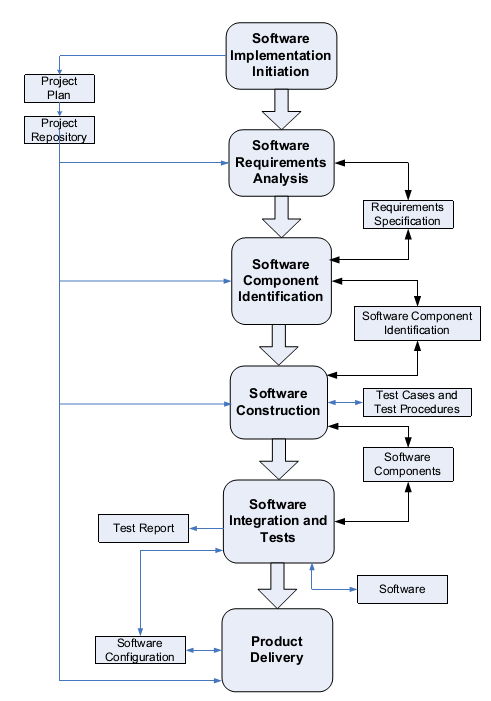
\includegraphics[width=.6\textheight]{SIprocess.png}$$
\end{frame}


\begin{frame}{Software Implementation}
\begin{itemize}
\item SI Output Documents
\begin{itemize}
\item Requirements Specification
\item Software Component Identification
\item Test Cases and Test Procedures
\item Software Components
\item Software Configuration
\item Software
\item Test Reports
\item Product Delivery
\item Acceptance Record
\end{itemize}
\item SI Internal Documents
\begin{itemize}
\item Change Request
\item Meeting Record
\item Progress Status Record
\end{itemize}
\end{itemize}
\end{frame}

\section{Oncloud Supporting Software}
\begin{frame}{www.hostedredmine.com}
\null
\kern -.5in
$$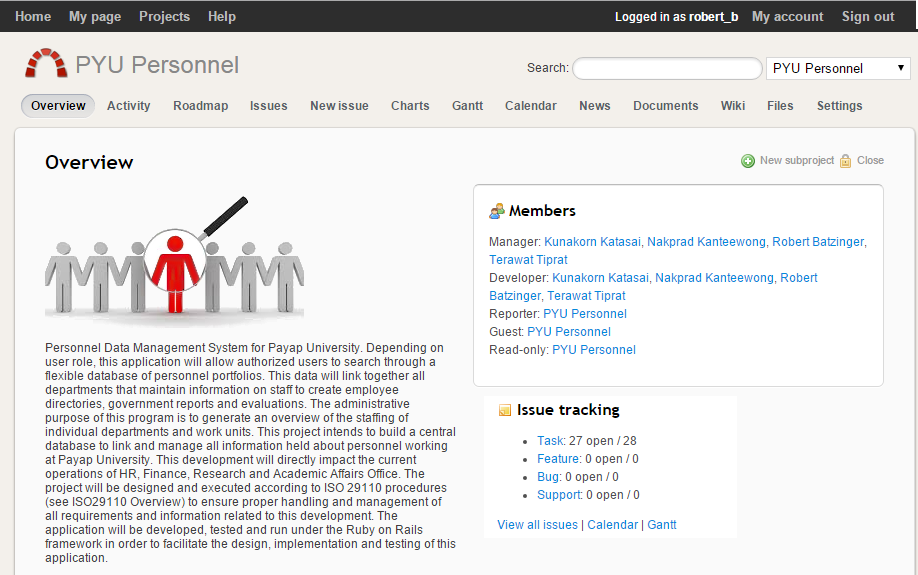
\includegraphics[width=.9\textheight]{redmine.png}$$
\end{frame}

\begin{frame}{www.gitlab.com}
\null
\kern -.5in
$$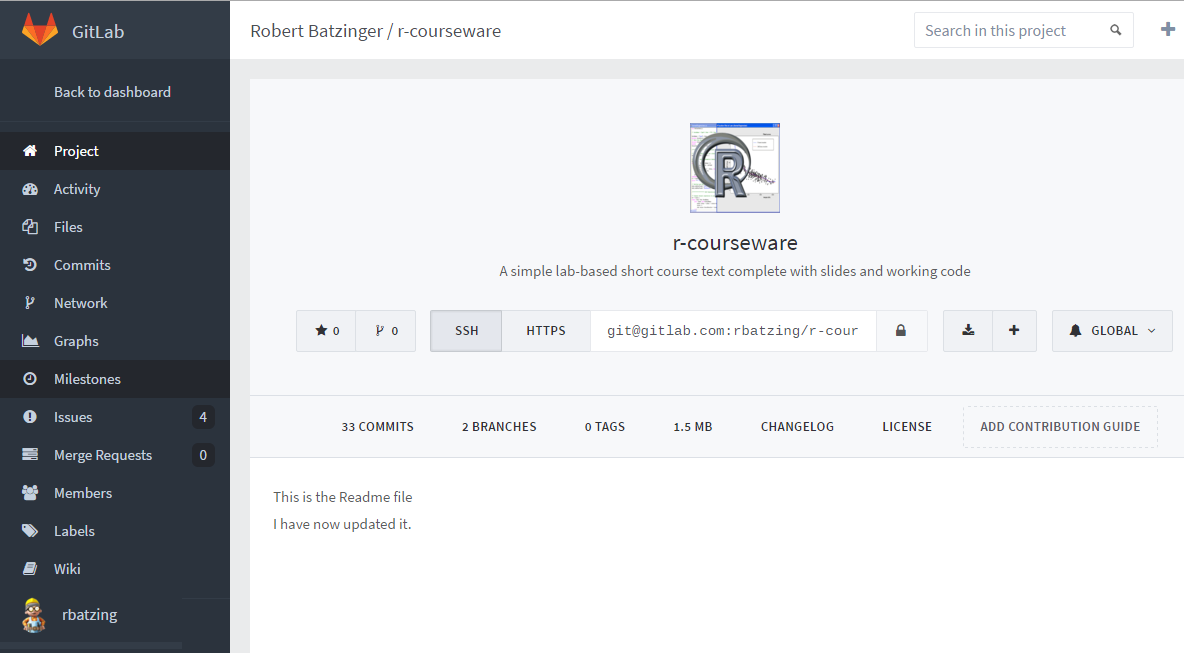
\includegraphics[width=.9\textheight]{gitlab.png}$$
\end{frame}

\begin{frame}{www.github.com}
\null
\kern -.5in
$$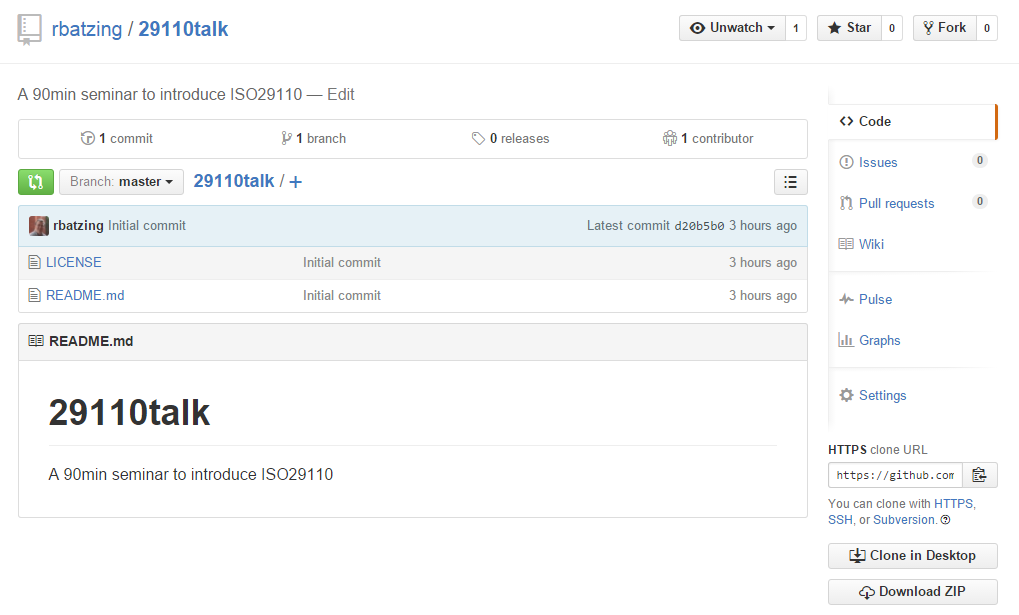
\includegraphics[width=.9\textheight]{github.png}$$
\end{frame}
\endinput

\section{Assignment}
\begin{frame}{Assignment}
\begin{itemize}
\item Select a team of 2 or 3 classmates
\item Sign up as a member for 2 of the online services mentioned.
\item Set up a simple project that will create software that will determine the sum of all odd numbers between 1 and 1000.
\item Use the wiki service to record the key aspects of the project relevant to ISO29110, namely:
\begin{itemize}
\item Statement of Work
\item Project Plan
\item Software Requirement
\item Pseudocode
\item Testing Plan
\item Test results
\item Software
\item Record of Acceptance
\end{itemize}
\item Compare the strengths and weakness of the two services you chose.
\item Indicate which one you would recommend for managing future projects
\end{itemize}

\end{document}

